\documentclass[t,12pt]{beamer}
\definecolor{links}{RGB}{0, 104, 172}
\definecolor{red}{rgb}{0.702,0.106,0.106} 
\hypersetup{colorlinks=true,urlcolor=links}
\usetheme{default}
% we need to change to Cornell red
\definecolor{beamer@blendedblue}{rgb}{0.702,0.106,0.106} 
\beamertemplatenavigationsymbolsempty
\setbeamerfont{institute}{size={\fontsize{10}{10}}}

\usepackage[english]{babel}
\usepackage{textgreek}
\usepackage{fontspec}
\setsansfont{TeX Gyre Heros}

\title{HD4630 Workshop II}
\subtitle{First- \& Second-Level Analysis}
\author{Elizabeth DuPre \\[.8\baselineskip]}

\vspace{2ex}
\institute{Human Neuroscience Institute 
\\[4pt]
\href{http://www.human.cornell.edu/hd/}{Department of Human Development}
\\[4pt]
\href{https://www.cornell.edu/}{Cornell University}}
\date{}

\begin{document}
% Title Slide
\begin{frame}
  \titlepage
\end{frame}

\section{Introduction}
% Slide
\begin{frame}{Workshop I Recap}
\vspace{10pt}
\begin{itemize}
\setlength\itemsep{1em}
\item Preprocessing 
\vspace{4pt}
\begin{itemize}
\setlength\itemsep{0.5em}
\item Discard pre-steady state TRs
\item Slice-timing correction
\item Rigid-body motion correction
\item Coregistration of functional \& anatomical
\item Normalization to standard template
\item Spatial filtering (Smoothing)
\end{itemize}
\item Quality Control
\vspace{4pt}
\begin{itemize}
\setlength\itemsep{0.5em}
\item Visual inspection
\item Censoring or "scrubbing" motion
\end{itemize}
\end{itemize}
\end{frame}

% Slide
\begin{frame}{Plan for Today}
\vspace{10pt}
\begin{itemize}
\setlength\itemsep{1em}
\item Discuss first- and second-level analyses in \\ a traditional general linear model (GLM) \\ framework
\item Conduct a first-level, fixed-effects analysis in AFNI using \texttt{uber\textunderscore{}subject.py}
\item Conduct a second-level, random-effects analysis in AFNI using \texttt{uber\textunderscore{}ttest.py}
\end{itemize}
\end{frame}

% Slide
\begin{frame}{First-level Analysis}
\vspace{10pt}
\begin{itemize}
\setlength\itemsep{1em}
\item First-level analysis involves estimating the \textbeta{}-matrix in
\begin{eqnarray*}
Y = X\beta + \epsilon
\end{eqnarray*}
by constructing the contrast matrix X
\item A great review of the math underlying this is available from \href{http://mumfordbrainstats.tumblr.com/post/125163337126/day-4-multiple-linear-regression}{Mumford Brain Stats}
\end{itemize}
\end{frame}

% Slide
\begin{frame}{First-Level Analysis, \textit{cont.}}
\vspace{10pt}
\begin{itemize}
\setlength\itemsep{1em}
\item We need to input the stimulus timing for each of the conditions in our task
\vspace{4pt}
\begin{itemize}
\item We'll collapse the two Flanker 'congruent' and 'incongruent' conditions, ignoring participant \\ accuracy
\end{itemize}
\end{itemize}
\vspace{4pt}
\centering
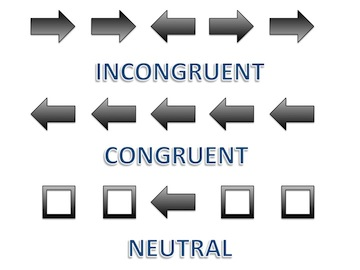
\includegraphics[width=.5\textwidth]{images/flanker_task.jpg}
\end{frame}

% Slide
\begin{frame}{}
\vspace{20pt}
\centering
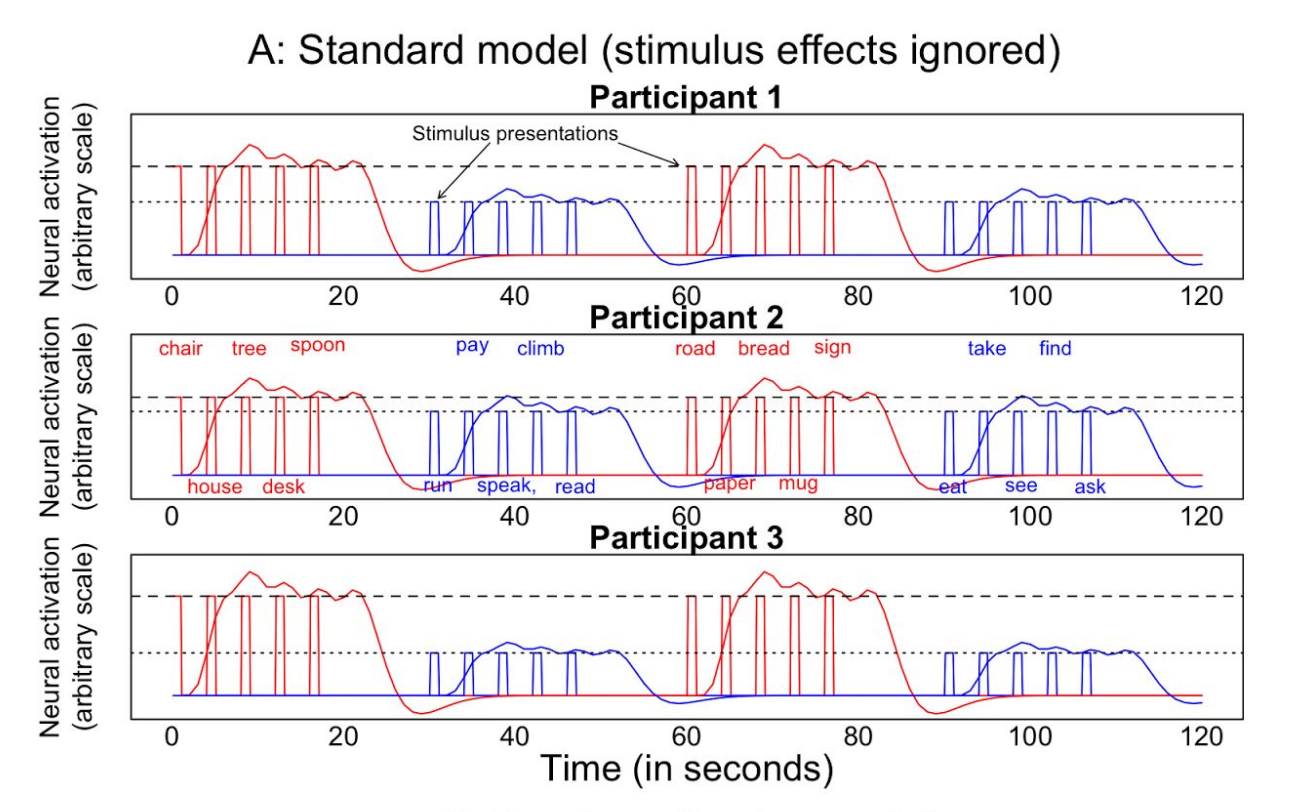
\includegraphics[width=\textwidth]{images/westfall_biorxiv.png} \\
\vspace{-10pt}
\begin{block}{}
Westfall, Nichols, \& Yarkoni \\ \href{http://biorxiv.org/content/early/2016/10/12/077131}{bioRxiv}
\end{block}
\end{frame}

% Slide
\begin{frame}{Second-Level Analysis}
\vspace{10pt}
\begin{itemize}
\setlength\itemsep{1em}
\item Second-level analysis as implemented in fMRI takes a summary-statistics approach
\begin{eqnarray*}
\hat{\beta} = X_{g}\beta_{g} + \eta^{*}
\end{eqnarray*}
where beta-hats for each contrast, for each subject are carried forward from the first-level
\item A great review of the math underlying this is available from \href{http://mumfordbrainstats.tumblr.com/post/128184717456/day-22-the-2-stage-summary-statistics-model-with}{Mumford Brain Stats}
\end{itemize}
\end{frame}

% Slide 
\begin{frame}{\emph{To Do}: Set Preprocessing Options}
\vspace{10pt}
\begin{itemize}
\setlength\itemsep{1em}
\item These were discussed in the last workshop
\vspace{4pt}
\begin{itemize}
\item For a review, see last week's slides on \\ the \href{https://emdupre.github.io/hd4630_workshops/categories}{course website}
\end{itemize}
\end{itemize}
\vspace{6pt}
\centering
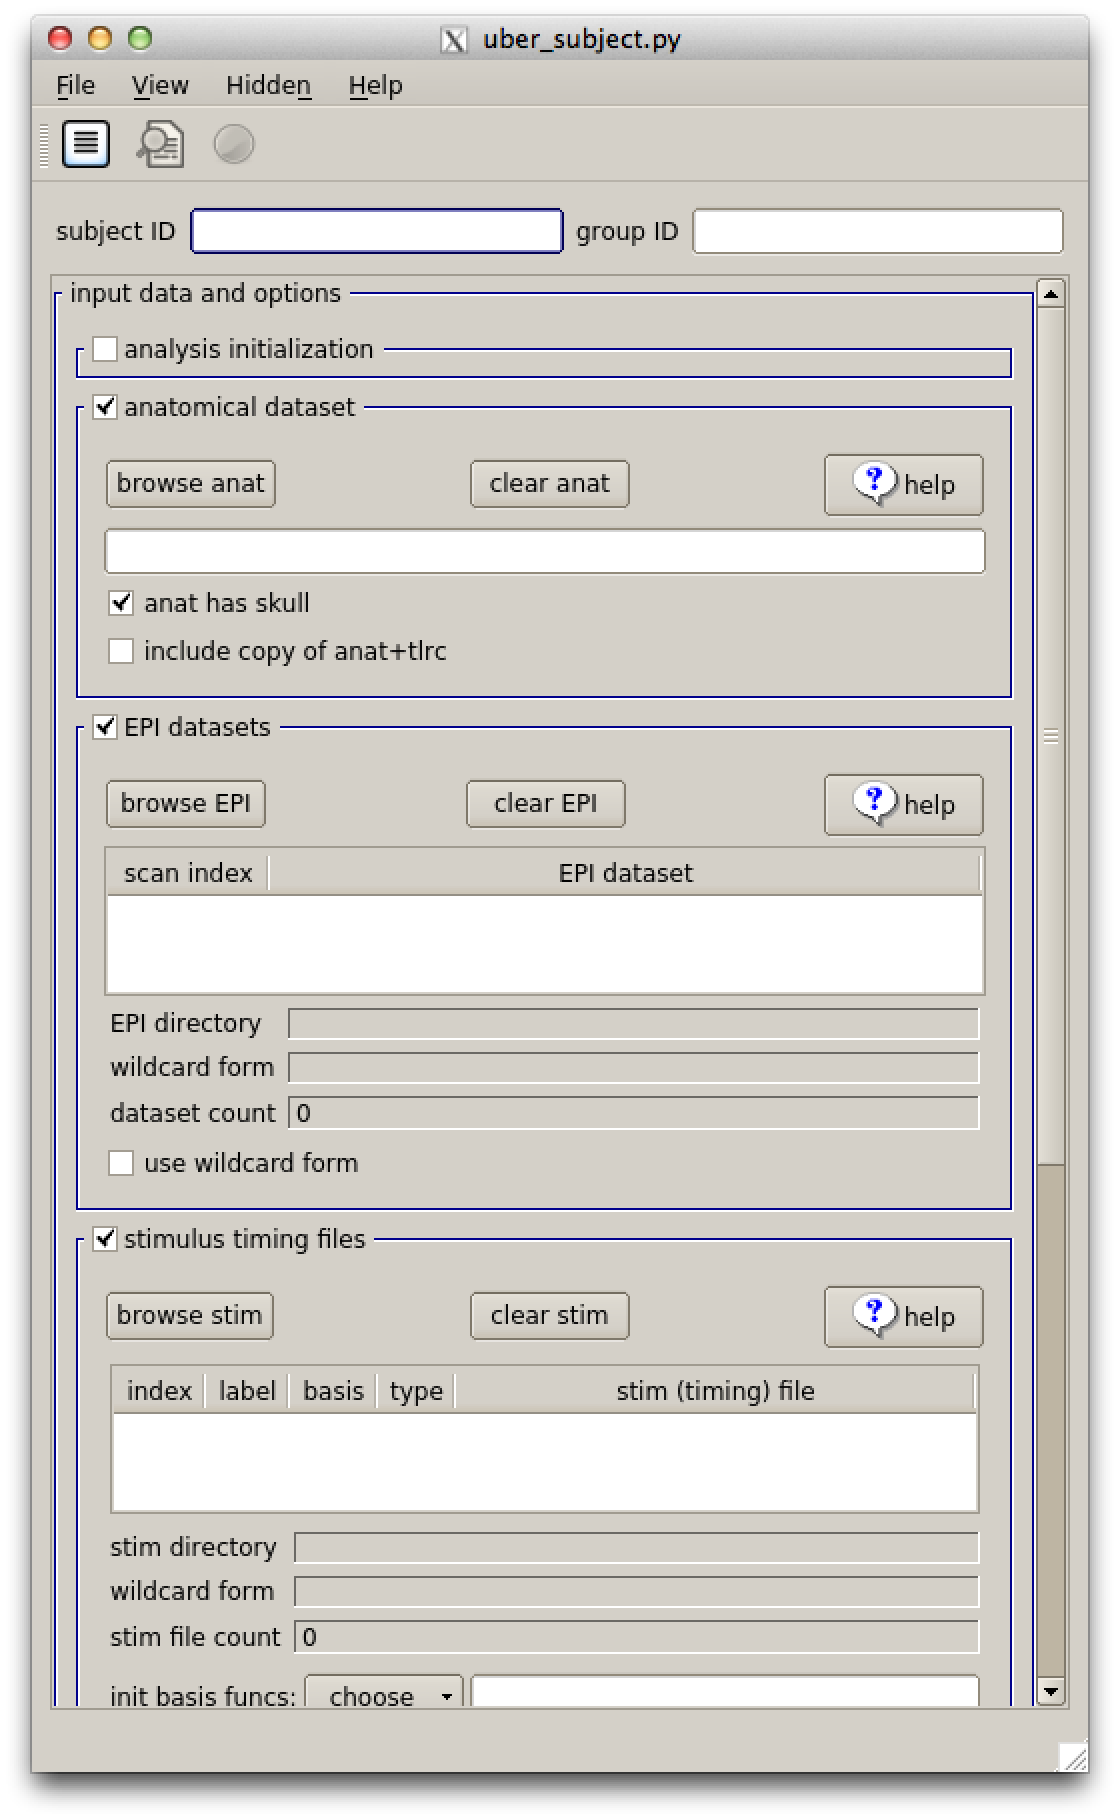
\includegraphics[width=.65\textwidth]{images/uber_subject.png}
\end{frame}

% Slide
\begin{frame}{Stimulus Timing Information}
\vspace{10pt}
\begin{itemize}
\setlength\itemsep{1em}
\item All stimulus timing information is included in the \texttt{*events.tsv} files for each run
\vspace{4pt}
\begin{itemize}
\item However, we need to convert this information into \\ text files that AFNI will accept
\end{itemize}
\item You'll be provided with a folder containing 
\vspace{4pt}
\begin{itemize}
\setlength\itemsep{0.5em}
\item A Python script to convert these files
\item The created text files themselves
\end{itemize}
\end{itemize}
\end{frame}

% Slide 
\begin{frame}{\emph{To Do}: Enter Stimulus Timing}
\vspace{10pt}
\begin{itemize}
\setlength\itemsep{1em}
\item In \texttt{uber\textunderscore{}subject.py}, select the provided text files in the section 'Stimulus Timing Files'
\item You can also specify the basis function and the file 'type' (see \texttt{3dDeconvolve -help} for relevant options)
\end{itemize}
\vspace{6pt}
\centering
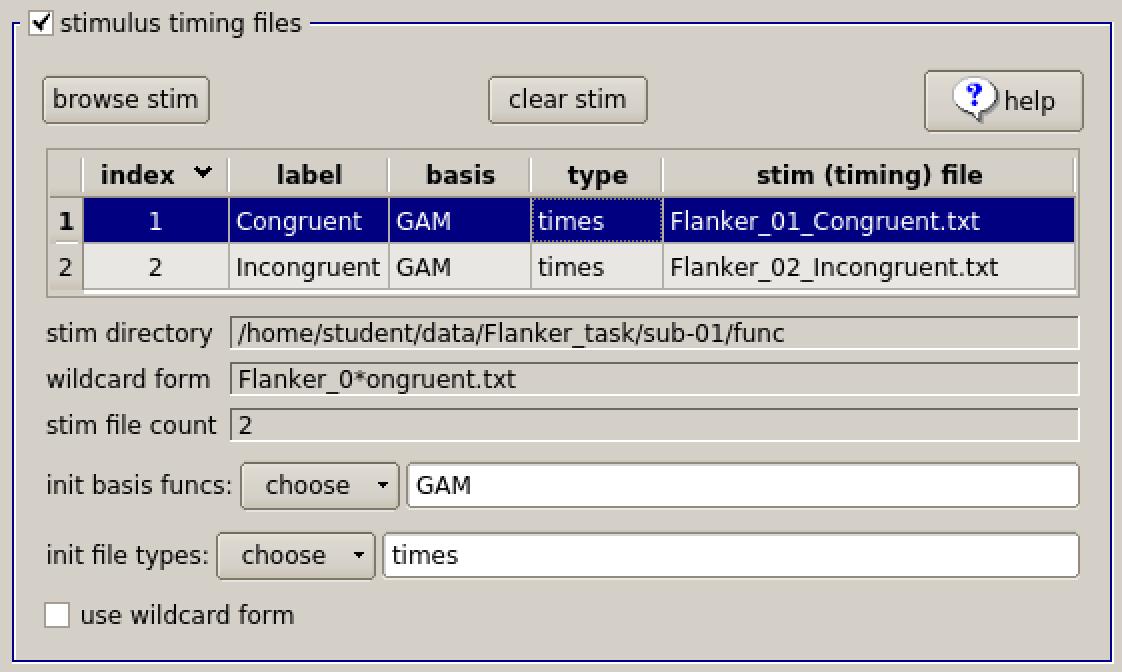
\includegraphics[width=.65\textwidth]{images/stimTime_spec.png}
\end{frame}

% Slide
\begin{frame}{General Linear Tests (GLTs)}
\vspace{10pt}
\begin{itemize}
\setlength\itemsep{1em}
\item AFNI refers to contrasts between conditions as General Linear Tests (GLTs)
\vspace{4pt}
\begin{itemize}
\item This is because we're working in the General \\ Linear Model (GLM)
\end{itemize}
\item We'll need to specify what tests we would like to conduct
\vspace{4pt}
\begin{itemize}
\item \textit{Congruent} > \textit{Incongruent} 
\item \textit{Incongruent} > \textit{Congruent} 
\end{itemize}
\end{itemize}
\end{frame}

% Slide 
\begin{frame}{\emph{To Do}: Specify GLTs}
\vspace{10pt}
\begin{itemize}
\setlength\itemsep{1em}
\item When inputting stimulus timing files, AFNI will automatically associate each condition with your provided label
\item You can use those labels to enter your desired GLTs
\vspace{4pt}
\begin{itemize}
\item Select 'init with examples' to see example GLTs with your conditions 
\end{itemize}
\end{itemize}
\vspace{6pt}
\centering
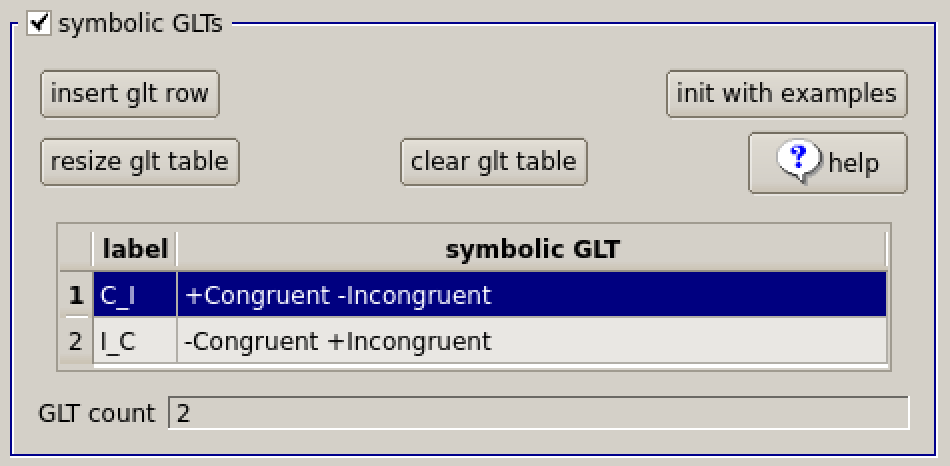
\includegraphics[width=.65\textwidth]{images/GLT_spec.png}
\end{frame}

% Slide
\begin{frame}{\emph{To Do}: Review Processing Script}
\vspace{10pt}
\begin{itemize}
\setlength\itemsep{1em}
\item Once you've entered all relevant parameters for preprocessing and first-level analysis, we can review and run the associated script
\item Estimated run time is 40 minutes per subject
\end{itemize}
\vspace{4pt}
\centering
\begin{minipage}{0.40\textwidth}
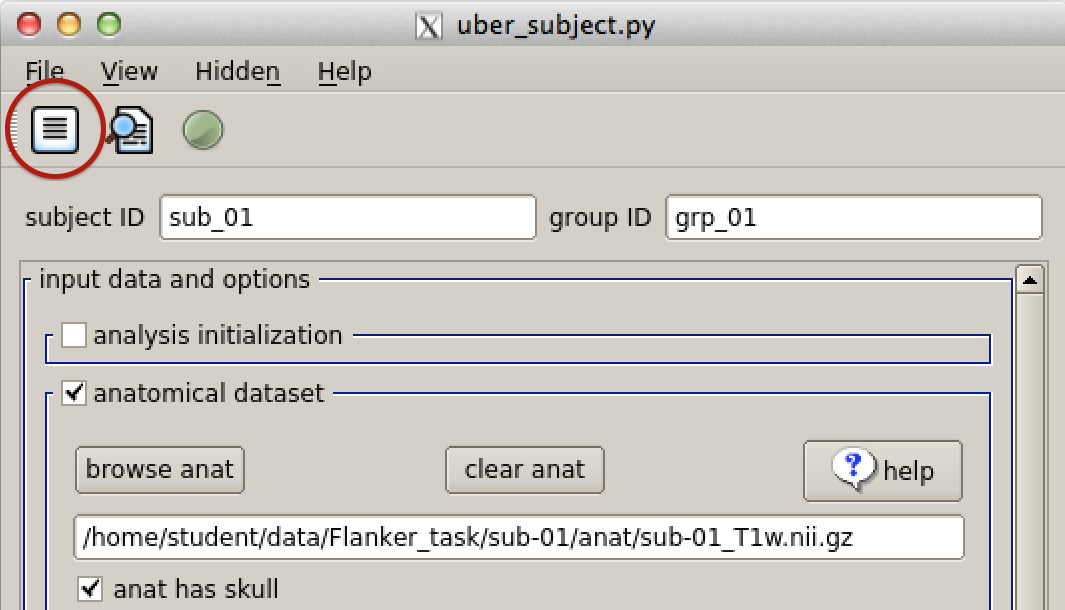
\includegraphics[width=\textwidth]{images/gen_afni_proc.png}
\end{minipage}
\begin{minipage}{0.55\textwidth}
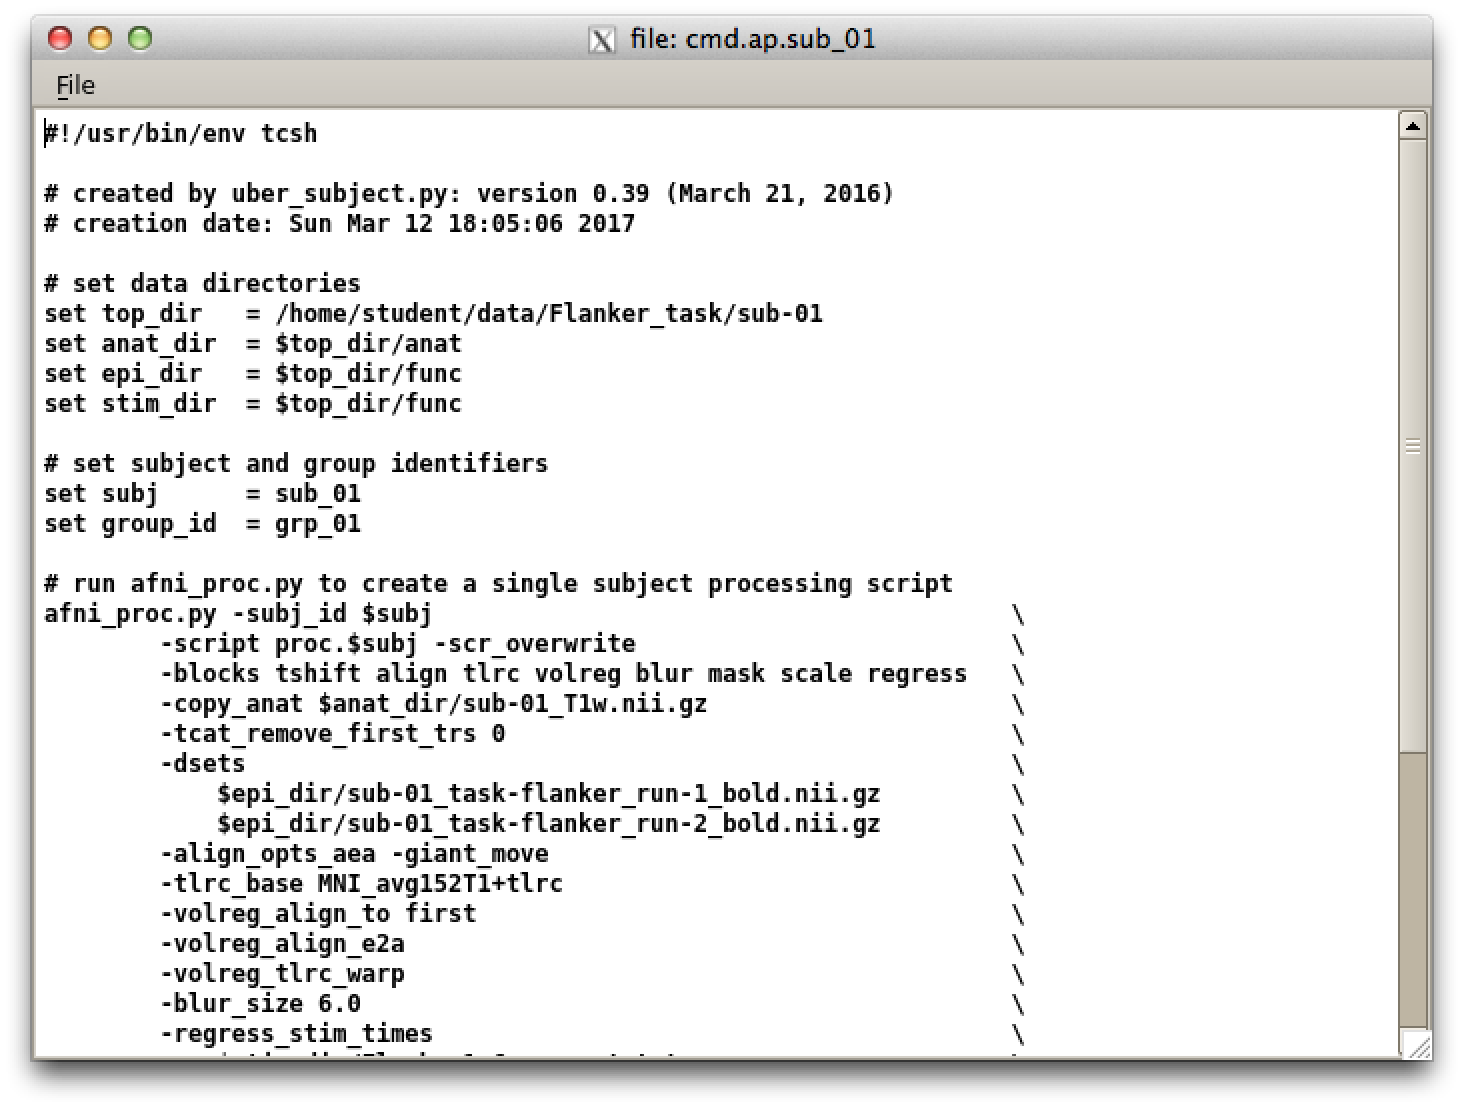
\includegraphics[width=\textwidth]{images/gen_script.png}
\end{minipage}
\end{frame}

% Slide
\begin{frame}{The Design Matrix}
\vspace{10pt}
\begin{itemize}
\setlength\itemsep{1em}
\item All of the information we have entered thus far will form the X or 'design' matrix
\item This is entered into the model 
\begin{eqnarray*}
Y = X\beta + \epsilon
\end{eqnarray*}
and will allow us to estimate the \textbeta{}-matrix for each participant
\end{itemize}
\end{frame}

% Slide
\begin{frame}{The Design Matrix, \textit{cont.}}
\vspace{10pt}
\begin{itemize}
\setlength\itemsep{1em}
\item After \texttt{uber\textunderscore{}subject.py}, the design matrix is output as a \texttt{*.xmat.1D} file
\item Multiple versions of this file exist, including
\vspace{4pt}
\begin{itemize}
\setlength\itemsep{0.5em}
\item A list of input stimulus timings \\ (\texttt{X.stim.xmat.1D})
\item A full design matrix with no motion censoring (\texttt{X.nocensor.xmat.1D})
\item A full design matrix with motion censoring (\texttt{X.xmat.1D})
\end{itemize}
\item In this class, we'll be working with the \texttt{X.xmat.1D} file
\end{itemize}
\end{frame}

% Slide
\begin{frame}{\emph{To Do}: Review the Design Matrix}
\vspace{10pt}
\begin{itemize}
\setlength\itemsep{1em}
\item \texttt{ExamineXmat} reads in the generated \texttt{*.xmat.1D} file \\ to visualize the time series of the design matrix
\item The generated X.jpg depicts a graph of the design matrix 
\vspace{4pt}
\begin{itemize}
\item You can recreate this using \texttt{1dgrayplot} to read in the \texttt{*.xmat.1D} file
\end{itemize}
\end{itemize}
\vspace{4pt}
\centering
\begin{minipage}{0.35\textwidth}
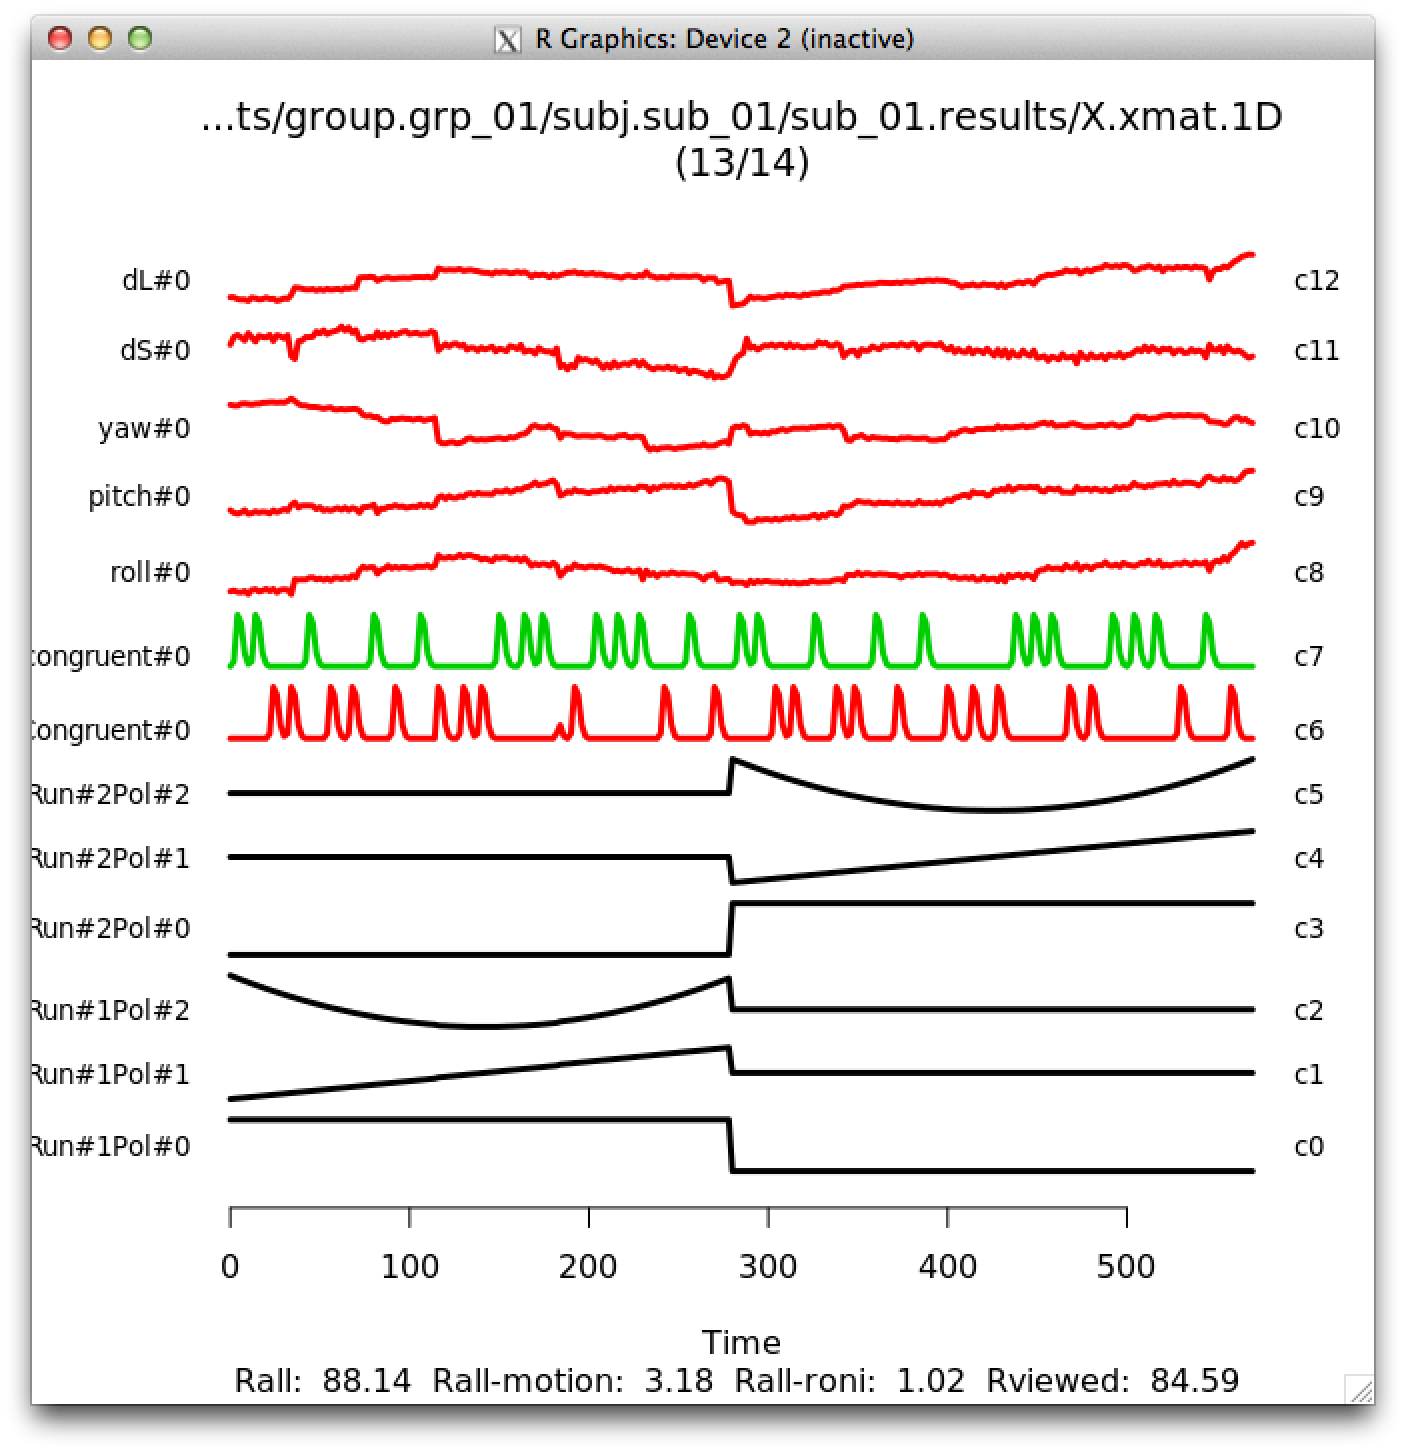
\includegraphics[width=\textwidth]{images/time_Xmat.png}
\end{minipage}
\begin{minipage}{0.30\textwidth}

\includegraphics[width=\textwidth]{images/X.jpg}
\end{minipage}
\end{frame}

% Slide
\begin{frame}{Pulling First-Level \textbeta{} Coefficients}
\vspace{10pt}
\begin{itemize}
\setlength\itemsep{1em}
\item We need to carry forward the beta coefficients from the first- to second-level
\vspace{4pt}
\begin{itemize}
\setlength\itemsep{0.5em}
\item We'll need their index in the created stats file to do that
\end{itemize}
\item To get the correct index, we can view our first-level results in AFNI
\end{itemize}
\end{frame}

% Slide
\begin{frame}{\emph{To Do}: View First-Level Results}
\vspace{10pt}
\begin{itemize}
\setlength\itemsep{1em}
\item Navigate to the output subject results directory \\ (e.g., \texttt{cd subj.sub\textunderscore{}01/sub\textunderscore{}01.results/})
\item Open \texttt{afni}
\vspace{4pt}
\begin{itemize}
\item You can also change the directory within AFNI using the 'Read' button
\end{itemize}
\end{itemize}
\vspace{4pt}
\centering
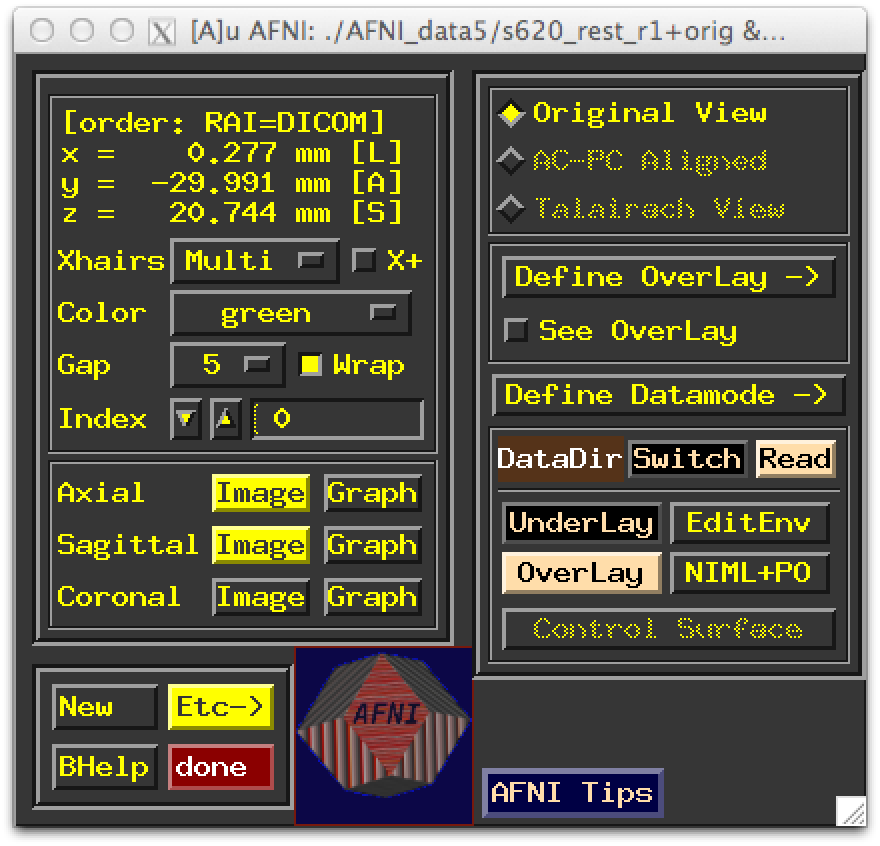
\includegraphics[width=0.45\textwidth]{images/afni_gui.png}
\end{frame}

% Slide
\begin{frame}{\emph{To Do}: View First-Level Results, \textit{cont.}}
\vspace{10pt}
\begin{itemize}
\setlength\itemsep{1em}
\item Once in AFNI, you can load the processed subject anatomical as an underlay \\ (e.g., \texttt{anat\textunderscore{}final.sub\textunderscore{}01})
\item Then load the first-level results as an overlay \\ (e.g., \texttt{stats.sub\textunderscore{}01})
\end{itemize}
\vspace{4pt}
\centering
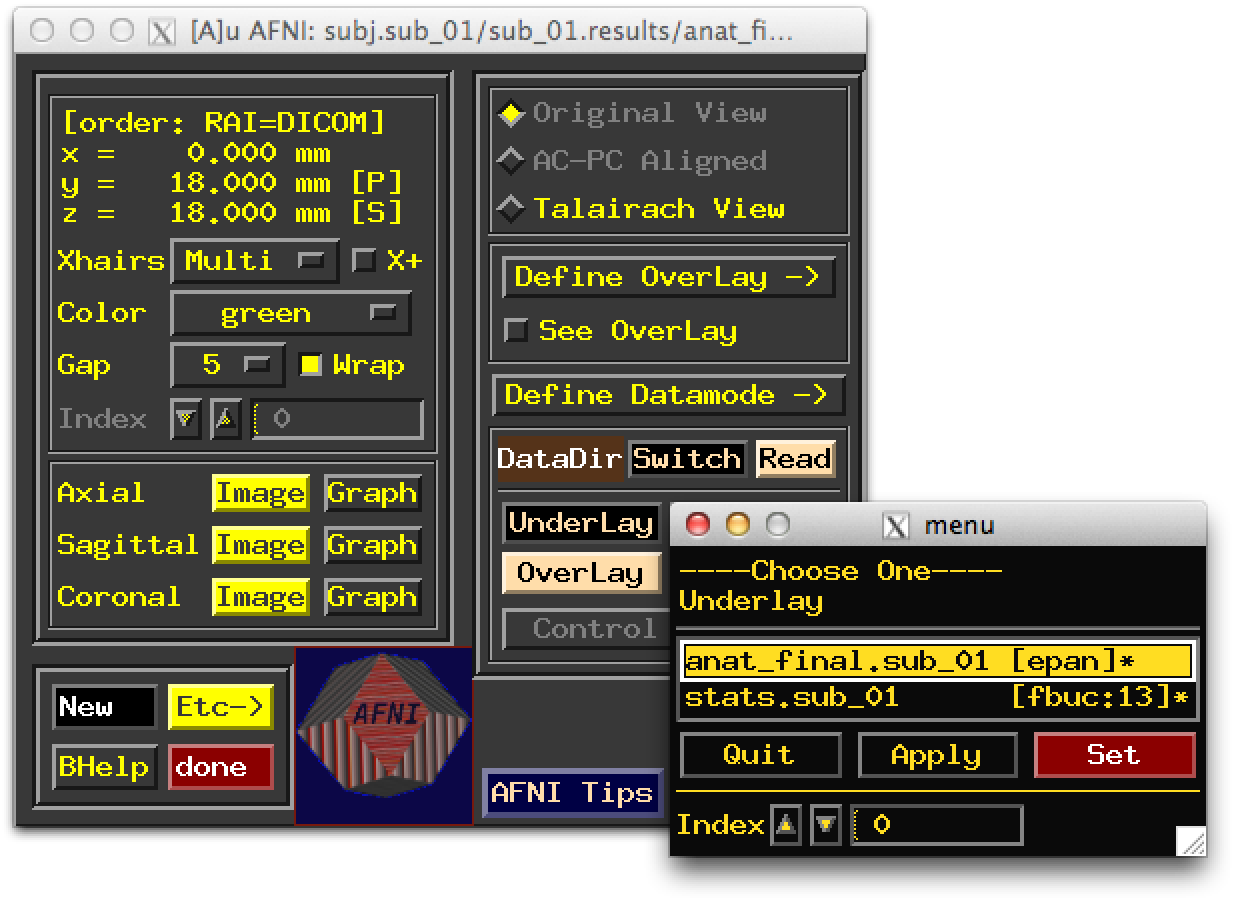
\includegraphics[width=0.6\textwidth]{images/select_underlay.png}
\end{frame}

% Slide
\begin{frame}{\emph{To Do}: View First-Level Results, \textit{cont.}}
\vspace{10pt}
\begin{itemize}
\setlength\itemsep{1em}
\item Click 'Define Overlay' to open the overlay menu
\item Hover over 'Olay;' it should read 'Choose overlay sub-brick' 
\item Clicking on 'Olay' will bring up a menu with the beta coefficients we created
\vspace{4pt}
\begin{itemize}
\setlength\itemsep{0.5em}
\item \textbf{Note the index} for the two GLTs \textbeta{} coefficients; in \\ the window below, they are 7 and 10
\end{itemize}
\end{itemize}
\vspace{4pt}
\centering
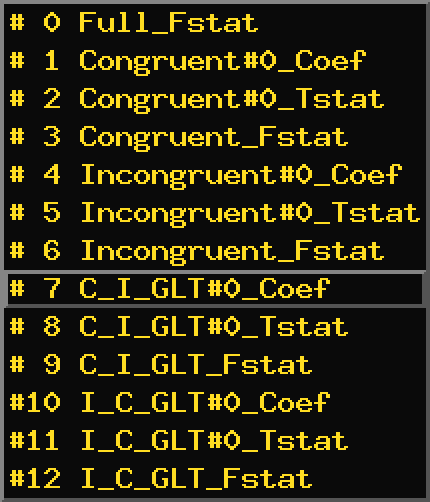
\includegraphics[width=0.25\textwidth]{images/olay.png}
\end{frame}

% Slide
\begin{frame}{Second-Level Analysis}
\vspace{10pt}
\begin{itemize}
\setlength\itemsep{1em}
\item Once we're confident at the first-level, we can move forward to second-level analysis
\item AFNI also provides a GUI to do this!
\vspace{4pt}
\begin{itemize}
\item \texttt{uber\textunderscore{}ttest.py}
\end{itemize}
\end{itemize}
\vspace{4pt}
\centering
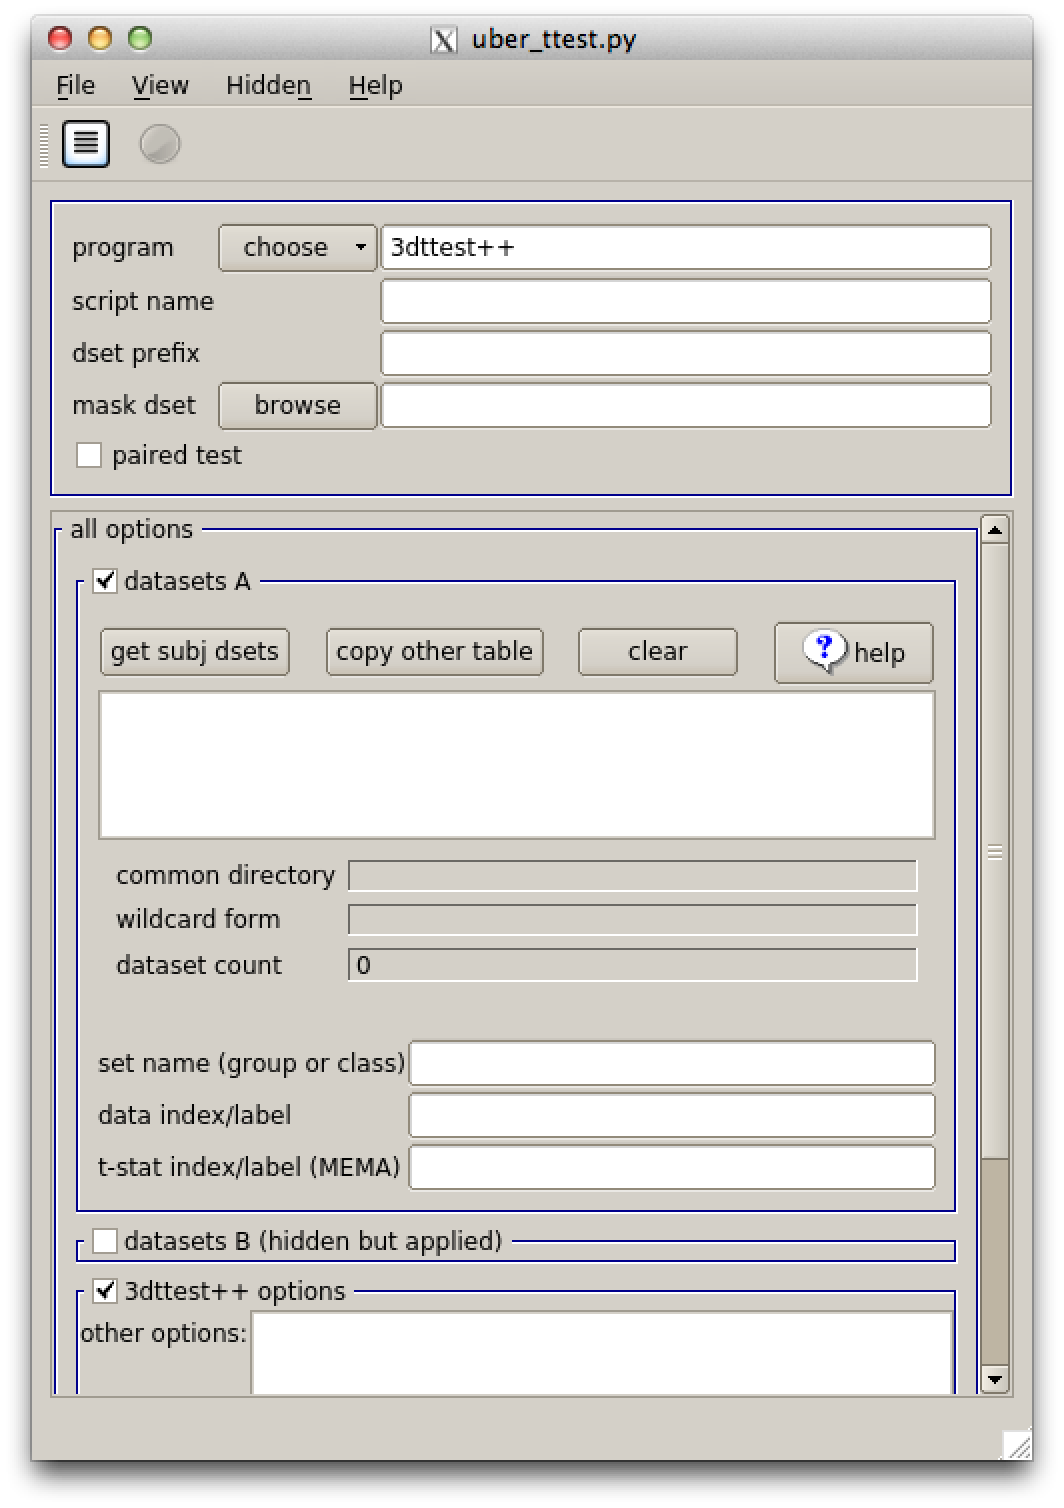
\includegraphics[width=.65\textwidth]{images/uber_ttest.png}
\end{frame}

% Slide
\begin{frame}{\emph{To Do}: Specify Second-Level}
\vspace{10pt}
\begin{itemize}
\setlength\itemsep{1em}
\item For each GLT, we need to conduct a second-level analysis
\item In \texttt{uber\textunderscore{}ttest.py}, the relevant parameters will be:
\vspace{4pt}
\begin{itemize}
\setlength\itemsep{0.5em}
\item 'dset prefix': the name of the GLT
\item 'subj dsets': the subject-specific stats files
\item 'group or class name': we'll set as 'subjs'
\item 'data index or label': the indices you noted previously
\end{itemize} 
\end{itemize}
\end{frame}

% Slide
\begin{frame}{\emph{To Do}: Specify Second-Level, \textit{cont.}}
\vspace{10pt}
\begin{itemize}
\setlength\itemsep{1em}
\item We need to populate our 'subj dsets' so they look like the table below (with stat files from all processed subjects) 
\item To do this, we'll create a wildcard pattern to match our subject-specific stat files
\end{itemize}
\vspace{4pt}
\centering
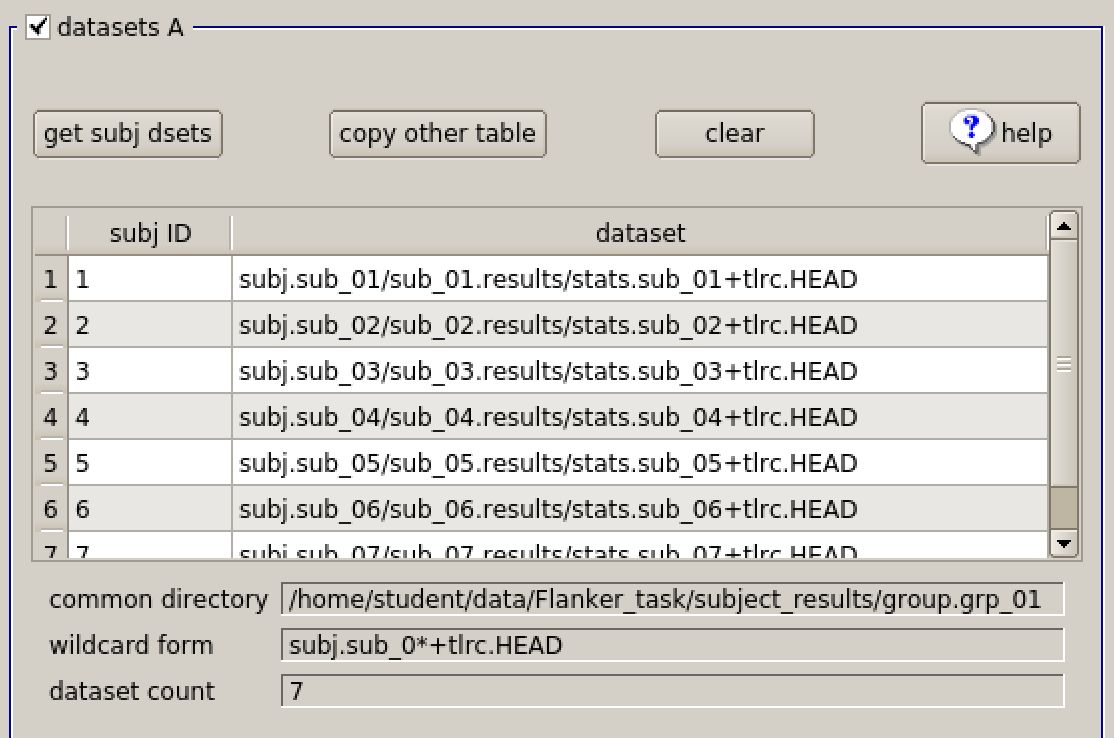
\includegraphics[width=.55\textwidth]{images/subj_dsets.png}
\end{frame}

% Slide
\begin{frame}{\emph{To Do}: Create Wildcard Pattern}
\vspace{10pt}
\begin{itemize}
\setlength\itemsep{1em}
\item Clicking on 'get subj dsets' will bring up a new menu
\item There, you can navigate to and select a stats file for one subject
\vspace{4pt}
\begin{itemize}
\item In the image below, I've selected a stats file for sub-01
\end{itemize}
\end{itemize}
\vspace{4pt}
\centering
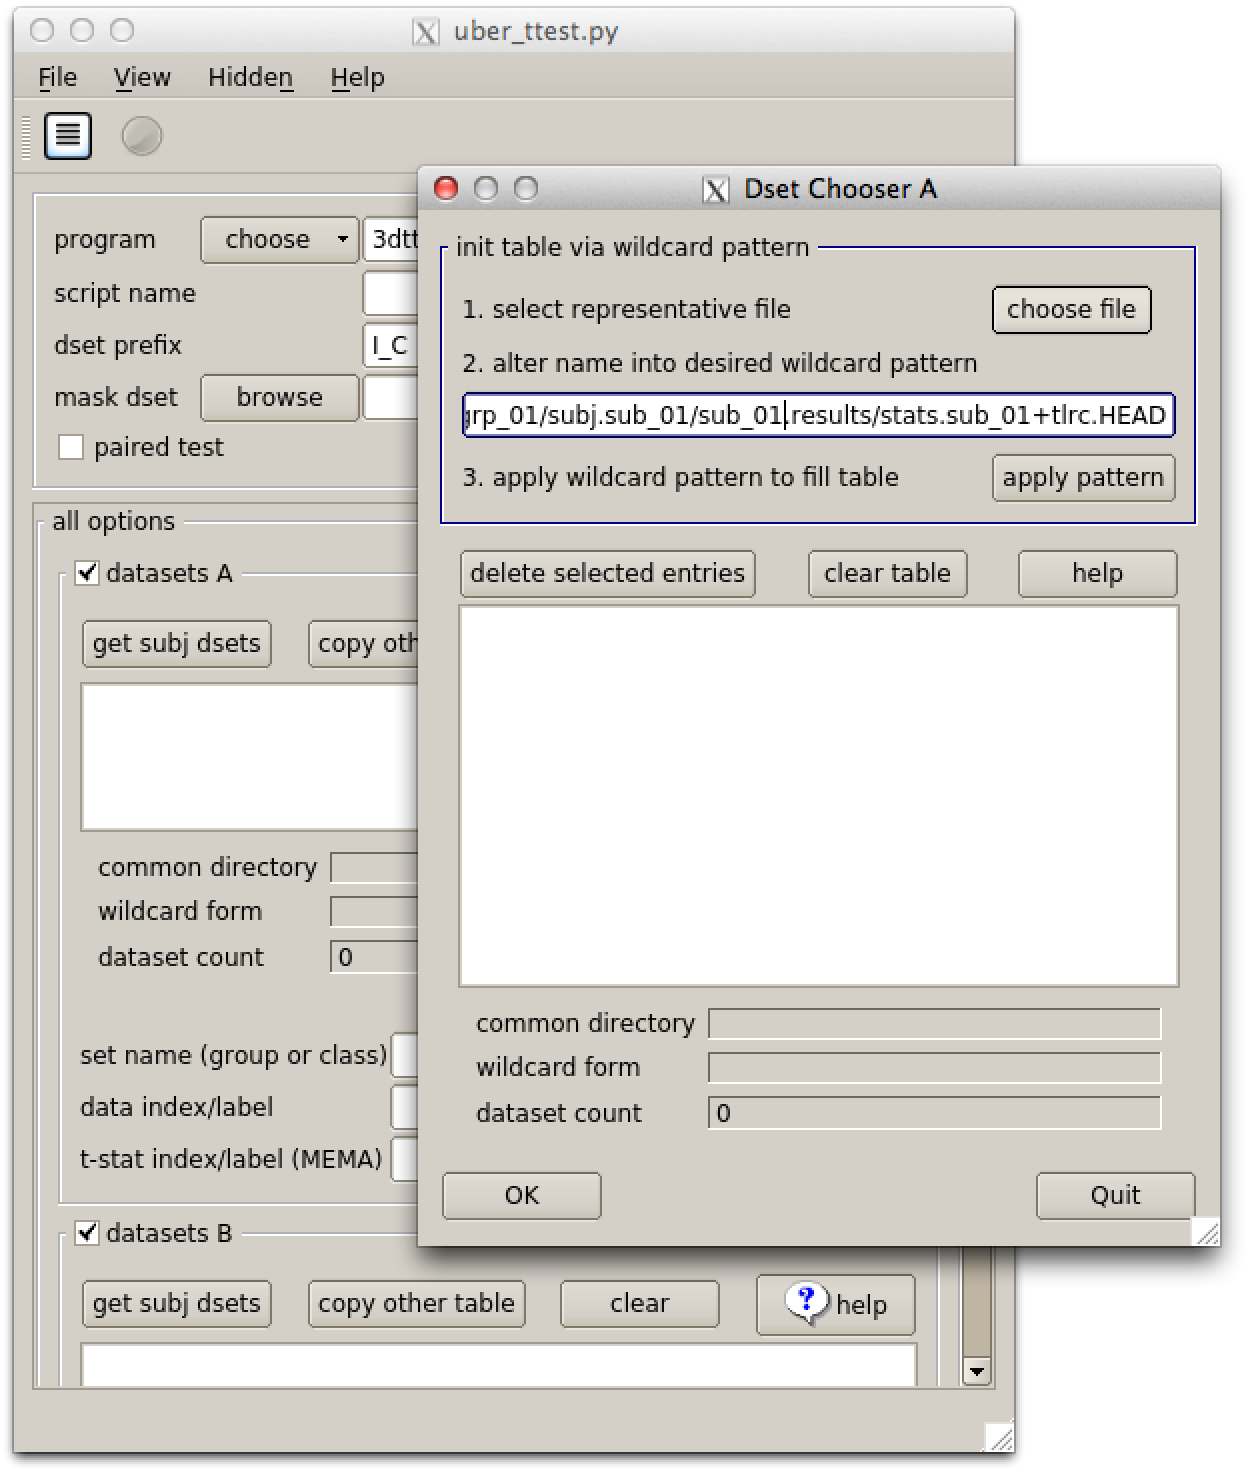
\includegraphics[width=.45\textwidth]{images/choose_rep_file.png}
\end{frame}

% Slide
\begin{frame}{\emph{To Do}: Create Wildcard Pattern, \textit{cont.}}
\vspace{10pt}
\begin{itemize}
\setlength\itemsep{1em}
\item Alter the name to be pattern, replacing subject-specific characters with question marks
\vspace{4pt}
\begin{itemize}
\item e.g., \texttt{sub\textunderscore{}01} becomes \texttt{sub\textunderscore{}??} 
\end{itemize}
\item Then click 'apply pattern'
\vspace{4pt}
\begin{itemize}
\item This should populate the table as below
\end{itemize}
\end{itemize}
\vspace{4pt}
\centering
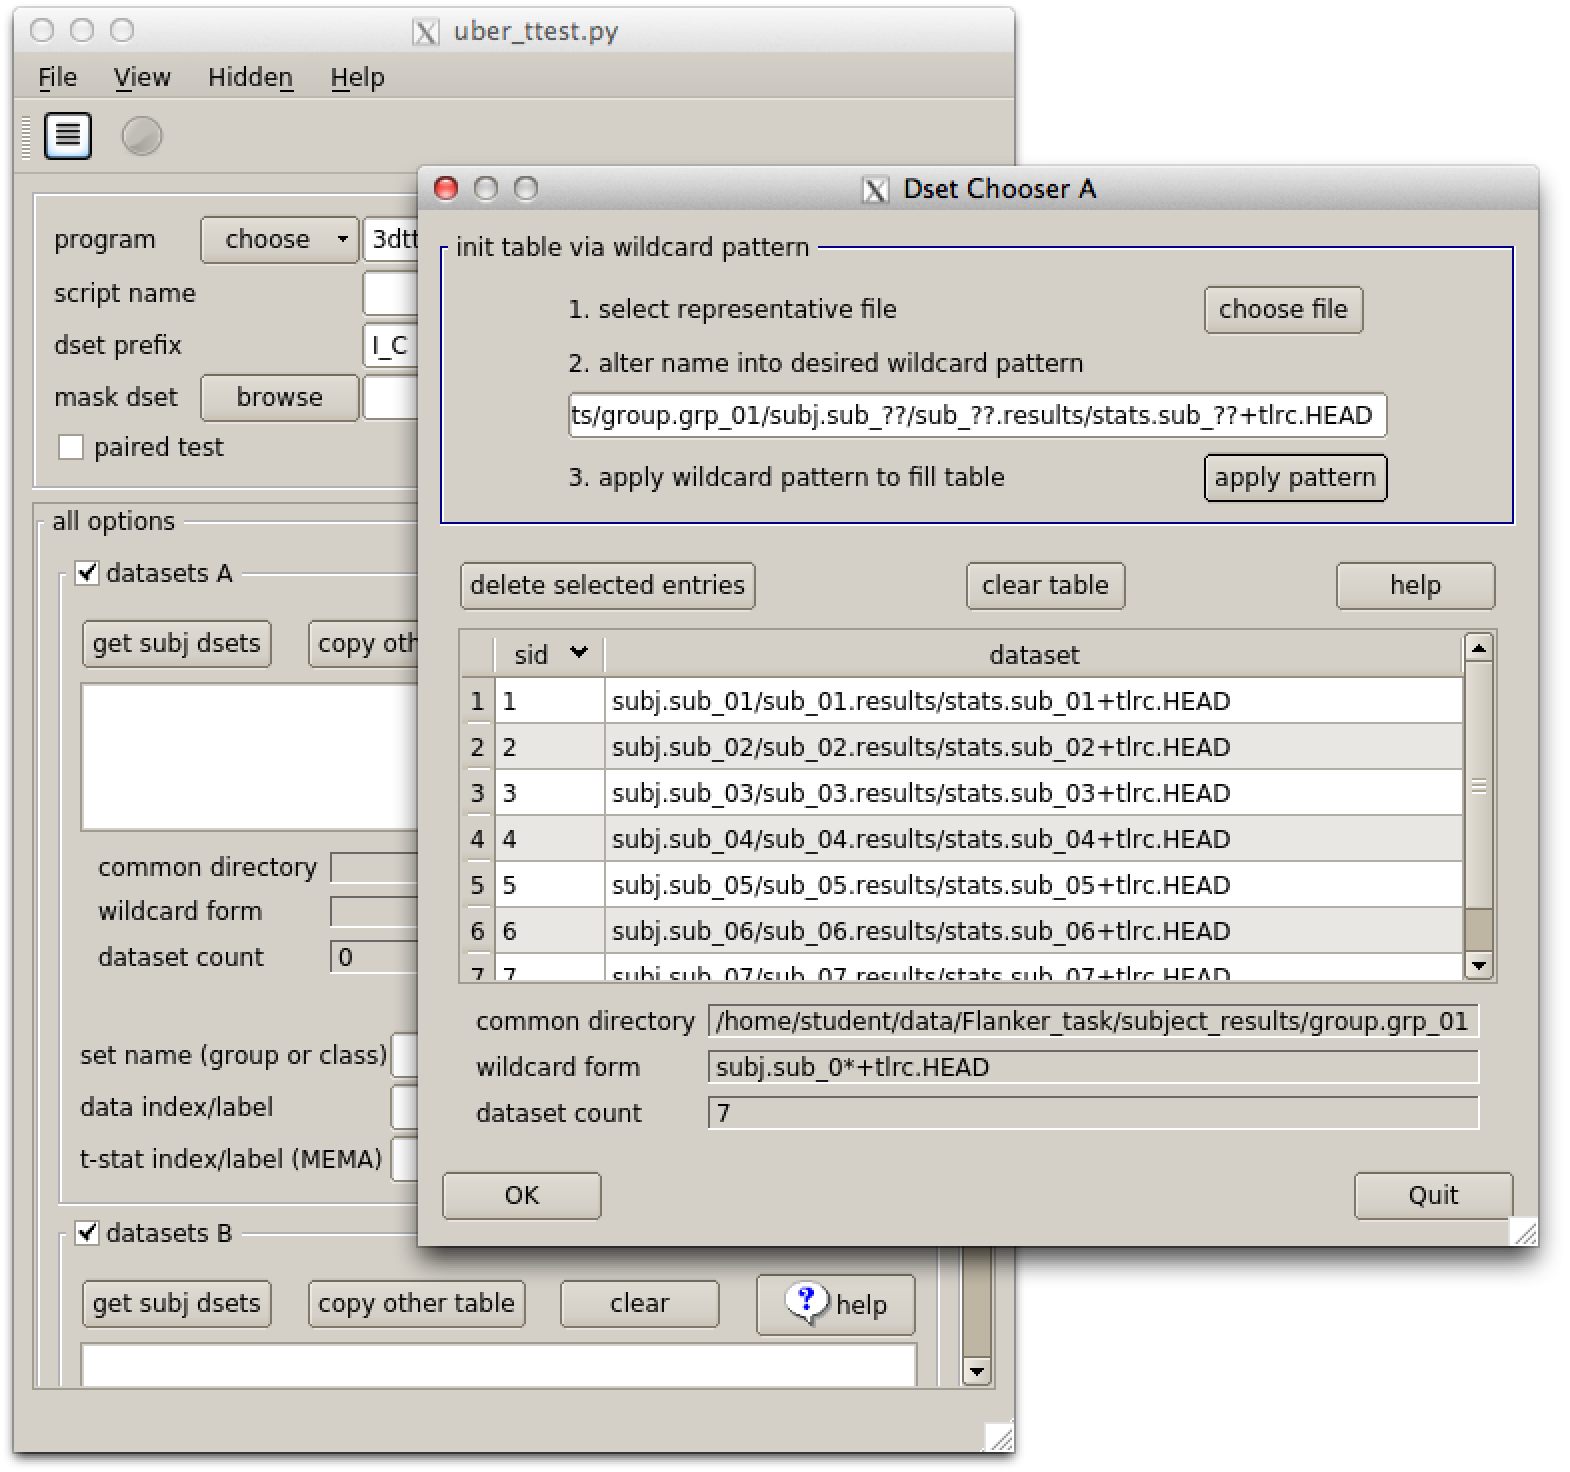
\includegraphics[width=.45\textwidth]{images/populated_subjs.png}
\end{frame}

\begin{frame}{\textit{To Do}: Run \texttt{uber\textunderscore{}ttest.py}}
\vspace{10pt}
\begin{itemize}
\setlength\itemsep{1em}
\item Review the generated \texttt{tcsh} script to be sure your indices were properly selected
\vspace{4pt}
\begin{itemize}
\item If you're satisfied with the parameters, run \\ it by clicking on the green circle as in \\ \texttt{uber\textunderscore{}subject.py}
\end{itemize}
\item For each GLT you conducted, you'll need to repeat \texttt{uber\textunderscore{}ttest.py}. For each test, you should edit
\vspace{4pt}
\begin{itemize}
\setlength\itemsep{0.5em}
\item The 'dset prefix' to the name of the GLT
\item The 'data index or label' to the index you noted in viewing first level results
\end{itemize}
\end{itemize}
\end{frame}

% Slide
\begin{frame}{Viewing Second-Level Results}
\vspace{10pt}
\begin{itemize}
\setlength\itemsep{1em}
\item Once we've run our second-level analysis using \texttt{uber\textunderscore{}ttest.py}, we need to view the results
\vspace{4pt}
\begin{itemize}
\item This will provide us information on which brain regions are active during each condition (e.g., \textit{Congruent} > \textit{Incongruent})
\end{itemize}
\item This can be done by navigating to the \texttt{group\textunderscore{}results} directory and launching \texttt{afni}
\vspace{4pt}
\begin{itemize}
\item Make sure you've previously copied in the desired template to the results folder(s) for each GLT!
\end{itemize}
\end{itemize}
\end{frame}

% Slide
\begin{frame}{\emph{To Do}: Load the Results}
\vspace{10pt}
\begin{itemize}
\setlength\itemsep{1em}
\item Load the template as an underlay as discussed in \textit{View First-Level Results}
\item Load the GLT second-level results image as an Overlay as discussed in \textit{View First-Level Results}
\vspace{4pt}
\begin{itemize}
\item The GLT second-level results will be named the 'dset prefix' you input into \texttt{uber\textunderscore{}ttest.py}
\end{itemize}
\end{itemize}
\end{frame}

% Slide
\begin{frame}{\emph{To Do}: Threshold the Results}
\vspace{10pt}
\begin{itemize}
\setlength\itemsep{1em}
\item After loading the image click on 'Define Overlay,' \\ then hover over the listed p-value (below the color bar)
\item Right-clicking on the p-value will bring up a menu where you can enter your desired threshold
\end{itemize}
\vspace{4pt}
\centering
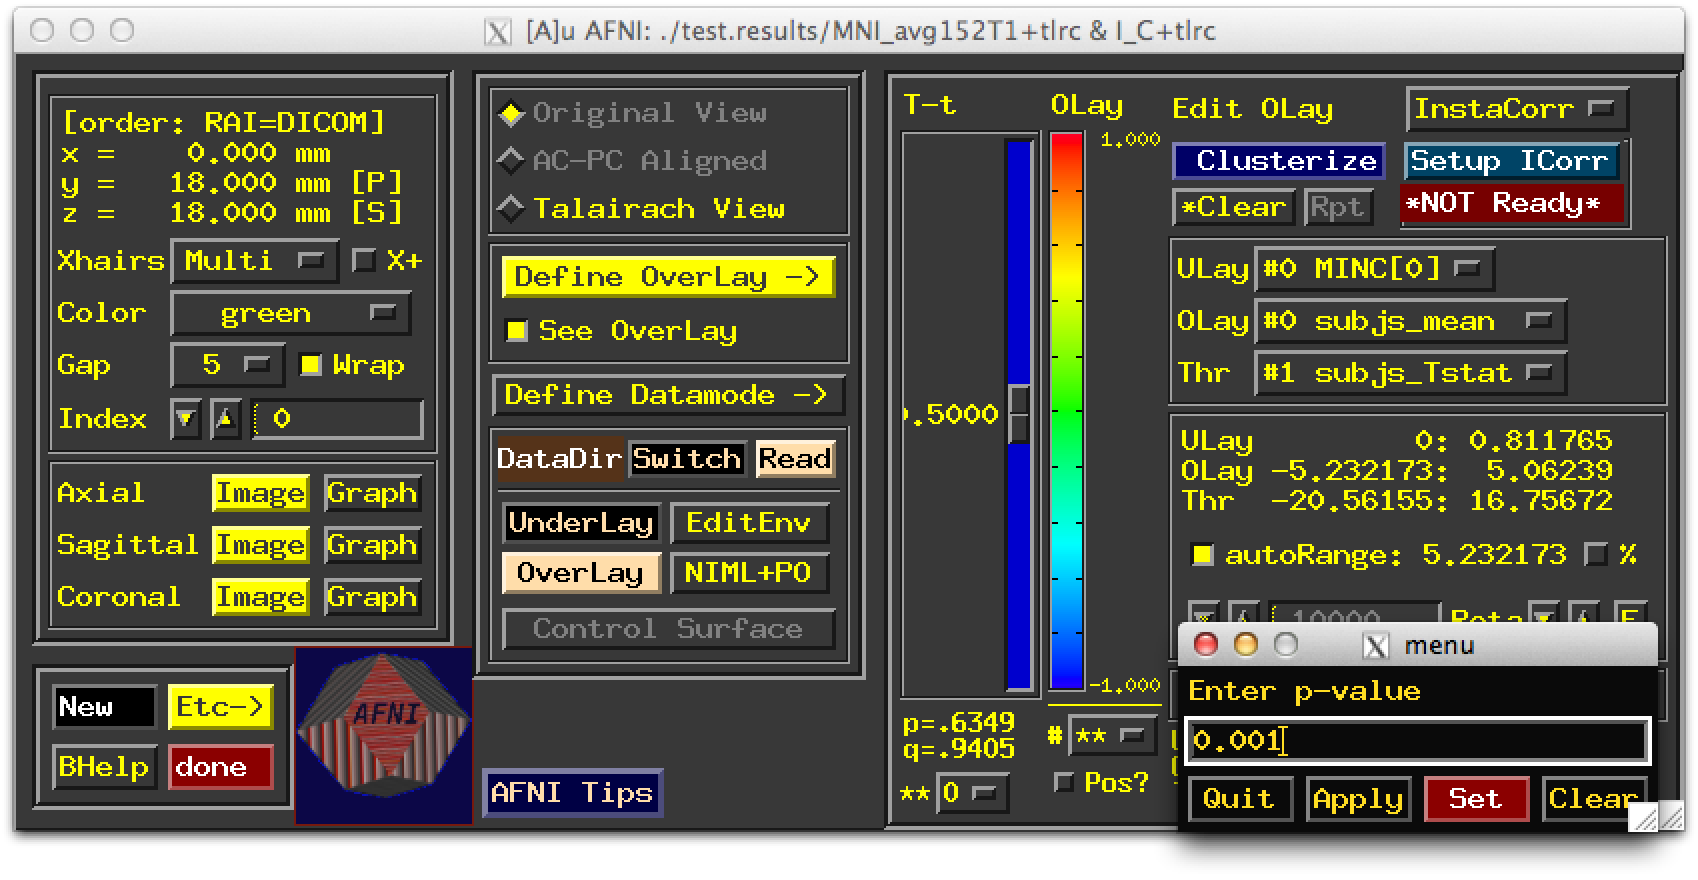
\includegraphics[width=.65\textwidth]{images/set_thresh.png}
\end{frame}

% Slide
\begin{frame}{\emph{To Do}: Threshold the Results, \textit{cont.}}
\vspace{10pt}
\begin{itemize}
\setlength\itemsep{1em}
\item We next need to set our cluster-threshold, or the number of contiguous voxels that must be in a cluster
\vspace{4pt}
\begin{itemize}
\item This is often reported as \textit{k}
\end{itemize}
\item Clicking on 'Clusterize' will load a menu where we can select our \textit{k} value-- the default is 20
\end{itemize}
\vspace{4pt}
\centering
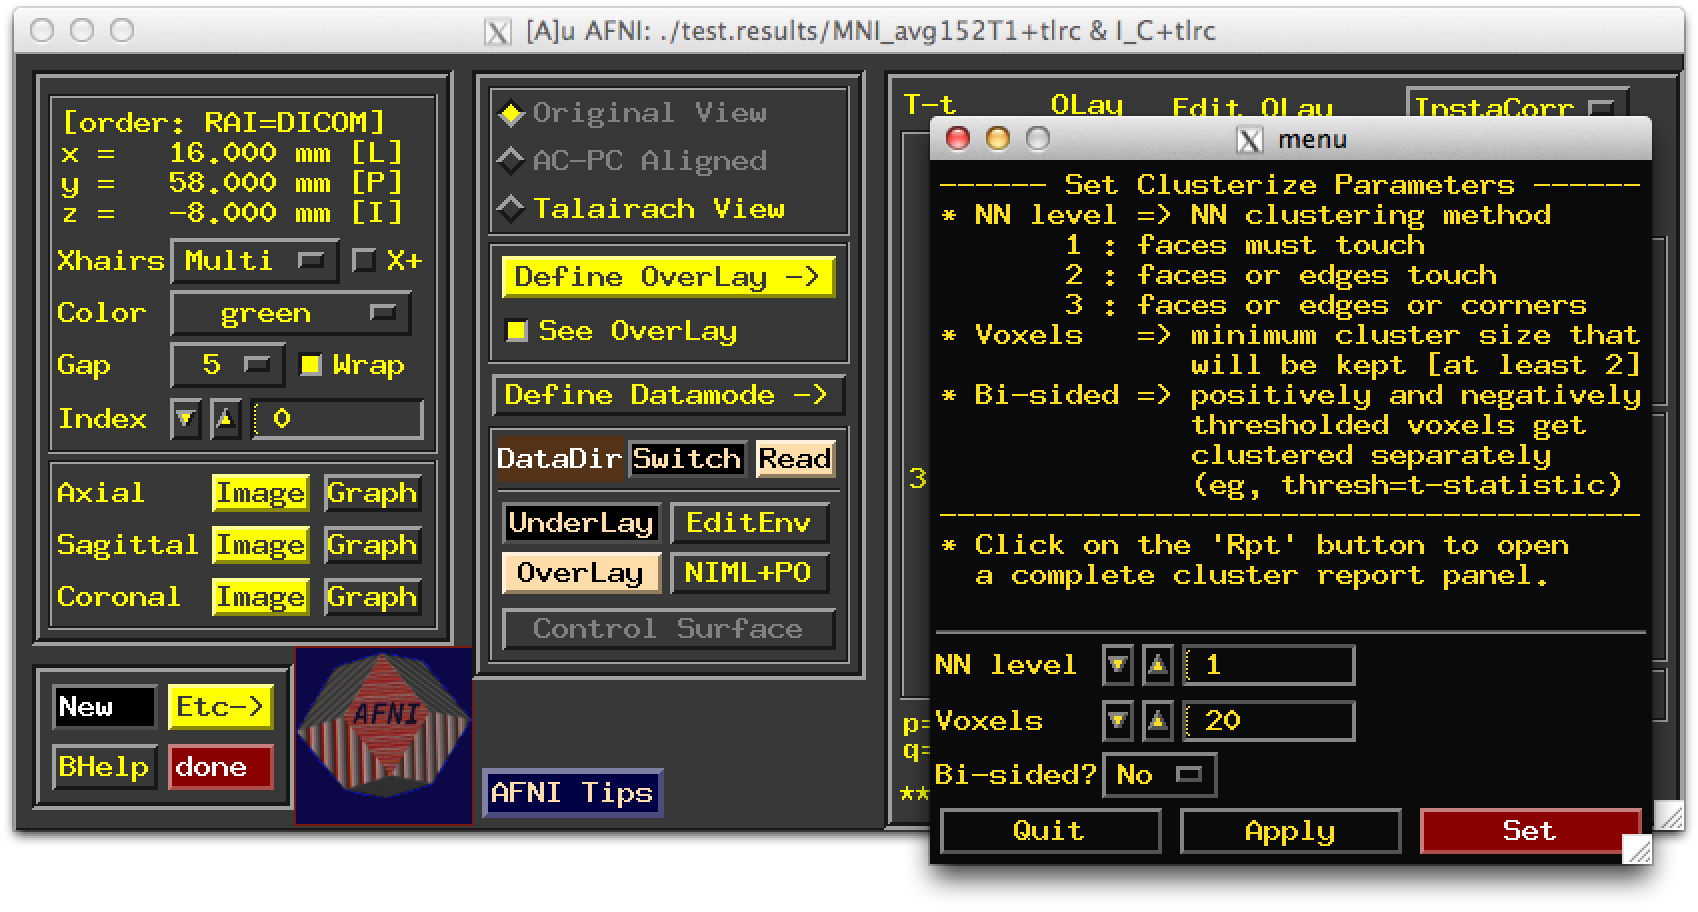
\includegraphics[width=.65\textwidth]{images/clusterize.png}
\end{frame}

% Slide
\begin{frame}{Reporting Second-Level Results}
\vspace{10pt}
\begin{itemize}
\setlength\itemsep{1em}
\item Once we have appropriately thresholded our results, we need to summarize them
\vspace{4pt}
\begin{itemize}
\item This is usually done by providing figures and tables
\end{itemize}
\end{itemize}
\end{frame}

% Slide
\begin{frame}{\emph{To Do}: Report Second-Level Results}
\vspace{10pt}
\begin{itemize}
\setlength\itemsep{1em}
\item Clicking on the 'Rpt' button under 'Clusterize' will generate a results table
\vspace{4pt}
\begin{itemize}
\setlength\itemsep{0.5em}
\item This can be used to jump to clusters for creating figures
\item The table itself can also be saved by clicking 'SaveTabl'
\end{itemize}
\end{itemize}
\centering
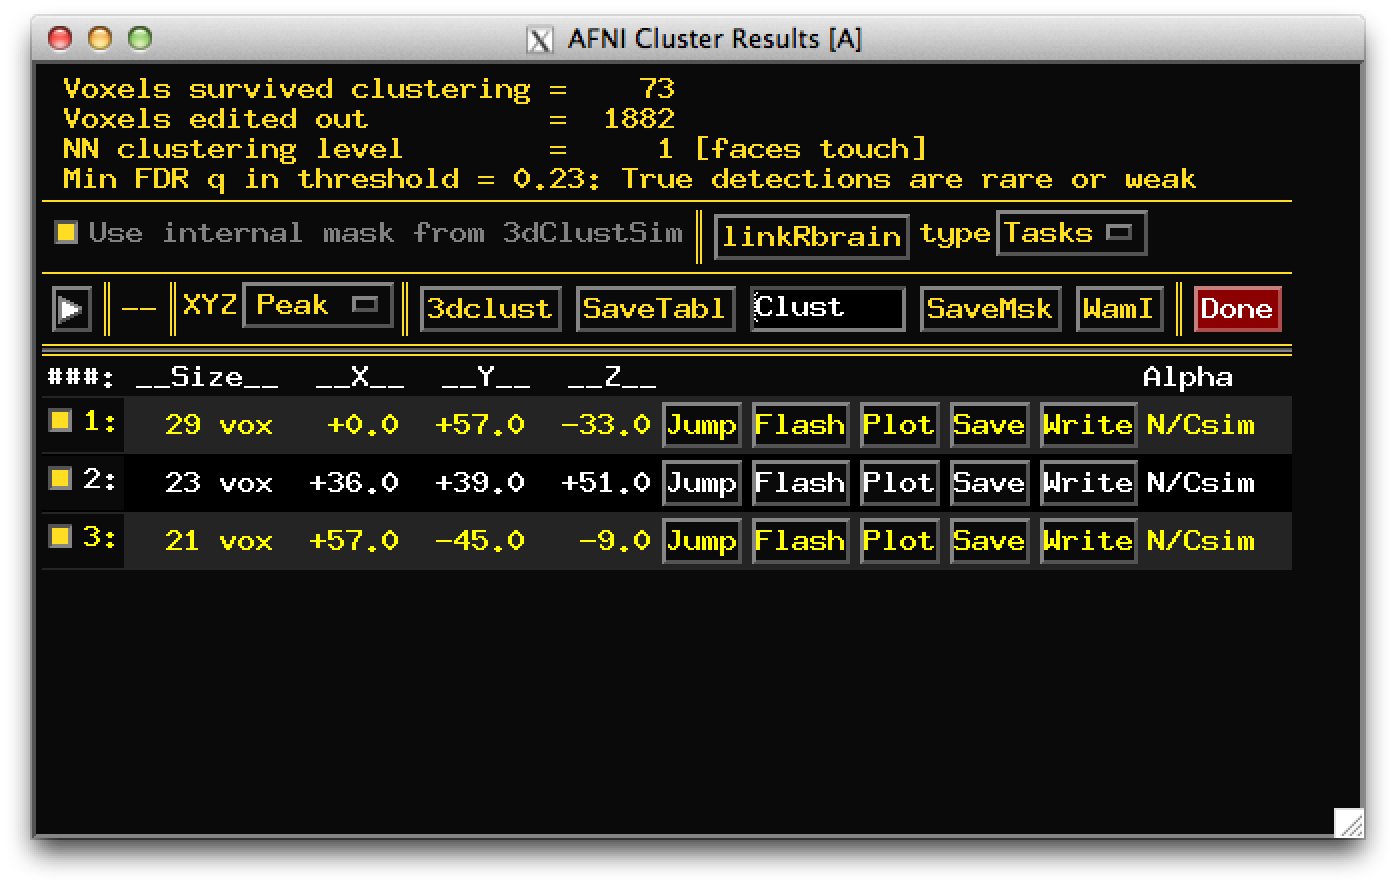
\includegraphics[width=.5\textwidth]{images/clust_rpt.png}
\end{frame}

\end{document}
